% DIPOLOMARBEITS TABELLEN DEUTSCH ########################
\newpage
\begin{center}
\textbf{\LARGE DIPLOMARBEIT}

\textbf{DOKUMENTATION}
\end{center}

\begin{tabular}{|p{53mm}|p{103mm}|@{}m{0cm}@{}}
\hline
\vspace{-0.11cm} Namen der \newline Verfasser/innen \vspace{0.11cm} & 
\vspace{-0.11cm} Clemens Schlipfinger\newline Felix Schneider \vspace{0.11cm}& \\
\hline
\vspace{-0.11cm} Jahrgang / Klasse \newline Schuljahr \vspace{0.11cm} & 
\vspace{-0.11cm} 5AHIT \newline 2023/24 \vspace{0.11cm} & \\
\hline
\vspace{-0.11cm} Thema der Diplomarbeit \vspace{0.11cm} & 
\vspace{-0.11cm} Visualisierung der Ergebnisse des Stromnetzmodells \vspace{0.11cm} & \\
\hline
\vspace{-0.11cm} Kooperationspartner \vspace{0.11cm} & 
\vspace{-0.11cm} Siemens AG Österreich \vspace{0.11cm} & \\
\hline
\end{tabular}

\vspace{0.5cm}

\begin{tabular}{|p{53mm}|p{103mm}|}
\hline
\vspace{-0.11cm} Aufgabenstellung \vspace{0.11cm} & 
\vspace{-0.11cm} Siemens entwickelt ein neues Programmpaket zur Echtzeitberechnung von Stromnetzwerken. Für diese Berechnung ist die Qualität des Netzmodells von höchster Wichtigkeit, aber aufgrund seiner Größe sind Fehler unvermeidlich. Aktuell werden Fehler in unübersichtlichen Log Files gespeichert. Ein ausfallsicheres System mit strukturierter Visualisierung wird für einfache Auswertungen benötigt. \vspace{0.11cm}  \\
\hline
\end{tabular}

\vspace{0.5cm}

\begin{tabular}{|p{53mm}|p{103mm}|}
\hline
\vspace{-0.11cm} Realisierung \vspace{0.11cm} & 
\vspace{-0.11cm} Die Applikation verwendet für das \emph{Backend} die Technologien \wordindoublequotes{Apache Kafka}, \wordindoublequotes{PostgreSQL} und das \wordindoublequotes{Java Spring}-\emph{Framework}. Die Schnittstelle zum \emph{Frontend} ist mit \wordindoublequotes{GraphQL} implementiert worden und das \emph{Frontend} selbst mit \wordindoublequotes{Angular}. \vspace{0.11cm} \\
\hline
\end{tabular}

\vspace{0.5cm}

\begin{tabular}{| p{53mm}|p{103mm}|}
\hline
\vspace{-0.11cm} Ergebnisse \vspace{0.11cm} & 
\vspace{-0.11cm} Das Projektziel ist die Entwicklung einer benutzerfreundlichen Webanwendung mit Filtermöglichkeiten, Graphen und Diagrammen. Dabei wird ein  Backend-System verwendet, welches durch die Verwendung von Apache Kafka reibungslos in die Siemens-Infrastruktur integriert werden kann und gleichzeitig höchste Stabilität und Fehlertoleranz  gewährleistet. Dadurch wird es den Siemens-Ingenieur:innen erleichtert, Netzmodellfehler zu analysieren. \vspace{0.11cm} \\
\hline
\end{tabular}
\newpage

\begin{tabular}{|p{53mm}|p{103mm}|}
\hline
\vspace{-0.11cm} Architektur der Applikation \vspace{0.11cm} &
\vspace{-0.11cm} 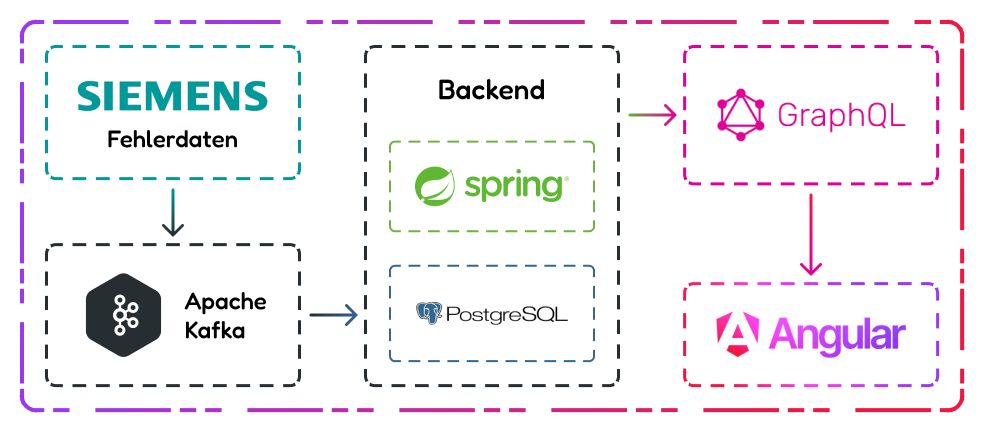
\includegraphics[width=0.62\textwidth]{content/img/Architecture/Architecture.jpg}
    Diese Grafik zeigt den Architekturaufbau unseres Prototypen. Die Daten werden vom System von Siemens AG über Apache Kafka in die PostgreSQL Datenbank gespeichert. Über die GraphQL API Schnittstelle stehen diese Daten dem Frontend zur Verfügung. \vspace{0.11cm} \\ 
\hline
\end{tabular}

\vspace{0.5cm}

\begin{tabular}{|p{53mm}|p{103mm}|}
\hline
\vspace{-0.11cm} Teilnahme an \newline Wettbewerben, \newline Auszeichnungen \vspace{0.11cm} &
\vspace{-0.11cm} Bosch Innovationspreis 2024 \vspace{0.11cm} \\
\hline
\end{tabular}

\vspace{0.5cm}

\begin{tabular}{|p{53mm}|p{103mm}|}
\hline
\vspace{-0.11cm} Möglichkeiten der \newline Einsichtnahme in die Arbeit \vspace{0.11cm} &
\vspace{-0.11cm} Der schriftliche Teil der Arbeit ist öffentlich einsehbar. Jedoch gibt es einen Sperrvermerk auf den Prototypen, da Siemens das Copyright auf den Programmcode besitzt. \vspace{0.11cm} \\
\hline
\end{tabular}

\vspace{0.5cm}

\begin{tabular}{|p{5.3cm}|p{4.93cm}|p{4.93cm}|@{}m{0cm}@{}}
\hline
\vspace{-0.11cm} Approbation \newline (Datum / Unterschrift) \vspace{0.11cm} & 
\vspace{-0.11cm} Prüfer/in  \vspace{0.11cm} &
\vspace{-0.11cm} Abteilungsvorstand / \newline Direktor/in \vspace{0.11cm} & \\ [4cm]
\hline
\end{tabular}